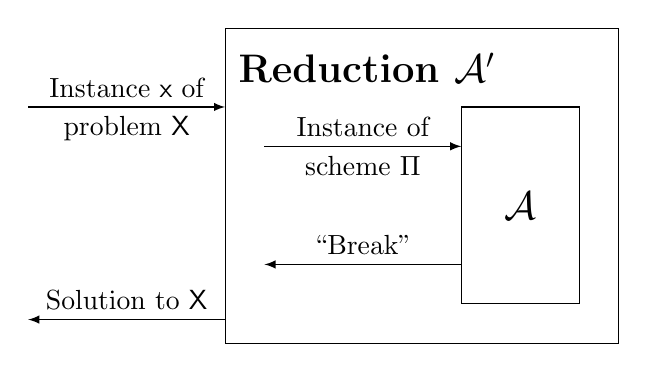
\begin{tikzpicture}
\draw (0,0) rectangle (5,4);
\draw (3,0.5) rectangle (4.5,3);
\draw[-latex] (-2.5,3) -- (0,3) node [midway, above] {Instance $\mathsf{x}$ of} node [midway, below] {problem $\mathsf{X}$};
\draw[-latex] (0,0.3) -- (-2.5,0.3) node [midway, above] {Solution to $\mathsf{X}$};
\draw (1.8,3.5) node {\Large \textbf{Reduction $\mathcal{A'}$}};
\draw (3.75,1.75) node {\Large $\mathcal{A}$};
\draw[-latex] (0.5,2.5) -- (3,2.5) node [midway, above] {Instance of} node [midway, below] {scheme $\Pi$};
\draw[-latex] (3,1) -- (0.5,1) node [midway, above] {``Break''};
\end{tikzpicture}